\documentclass[a4paper]{article}

\usepackage[a4paper, total={7in, 10in}]{geometry}
\usepackage[T1,T2A]{fontenc}
\usepackage[utf8]{inputenc}
\usepackage[english,russian]{babel}
\usepackage{graphicx}
\usepackage{enumitem}
\usepackage{tcolorbox}
\tcbuselibrary{listings,skins}

\graphicspath{ {./images/} }

\begin{document}

\title{\textit{\textbf{Лабораторная работа №1}}}
\author{Губанов Пётр, С01-019}
\maketitle

\clearpage

\begin{enumerate}[label=\arabic*.]
\item Запустим программу по выводу регистра esp с включенным ASLR.
\end{enumerate}

\begin{center}
	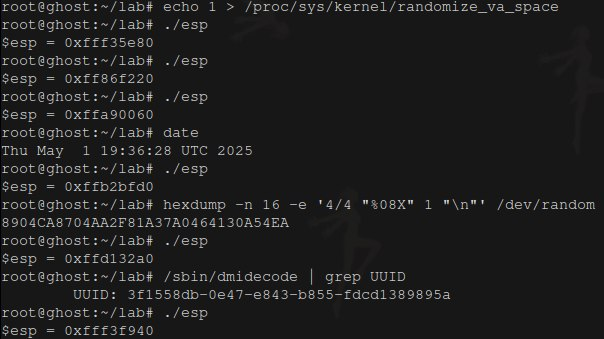
\includegraphics[scale=1]{./images/1.jpg}
\end{center}

\begin{enumerate}[resume]
	\item Запустим программу по выводу регистра esp с выключенным ASLR.
\end{enumerate}

\begin{center}
	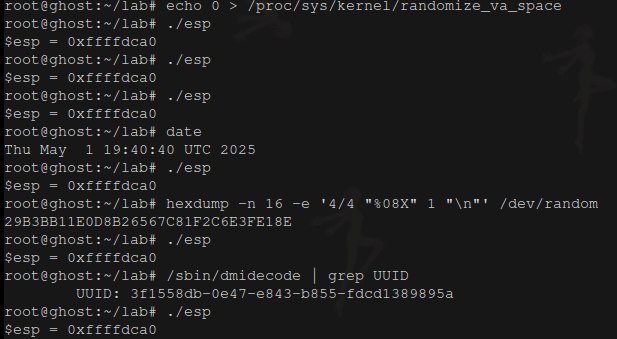
\includegraphics[scale=1]{./images/2.jpg}
\end{center}

\begin{enumerate}[resume]
\item Попытаемся скомпилировать предоставленный код.
\end{enumerate}

\begin{tcblisting}{colback=white, colframe=black!70, listing only, title=Вывод компилятора, fonttitle=\bfseries}
root@ghost:~/lab# gcc -g -m32 -z execstack -no-pie -o bo1 bo1.c -mpreferred-stack-boundary=4

bo1.c: In function 'main':
bo1.c:4:2: warning: implicit declaration of function 'copier'; did you mean 'popen'? [-Wimplicit-function-declaration]
  copier(argv[1]);
  ^~~~~~
  popen
\end{tcblisting}

\begin{enumerate}[resume]
	\item Программа успешно скомпилировалась. Однако, компилятор не может найти функцию с названием copier. Всё потому что её сигнатура объявлена позже первого использования. Корректным исправлением будет добавление прототипа функции в самом начале. Таким образом получится:
\end{enumerate}


\begin{tcblisting}{colback=white, colframe=black!70, listing only, title=Исправленный код, fonttitle=\bfseries}
#include <string.h>
#include <stdio.h>

int copier(char *str);

void main(int argc, char *argv[]) {
        copier(argv[1]);
        printf("Done!\n");
}

int copier(char *str) {
        char buffer[100];
        strcpy(buffer, str);
}
\end{tcblisting}

Флаг компилятора \texttt{-mpreferred-stack-boundary=4} устанавливает выравнивание стека на $2^4=16$ байт.

\begin{center}
	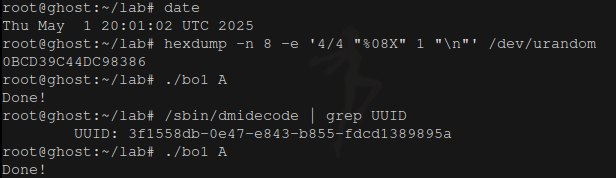
\includegraphics[scale=1]{./images/3.jpg}
\end{center}

\begin{enumerate}[resume]
	\item Причина возникновения ошибки \texttt{Segmentation fault (core dumped)} в том, что мы смогли перезаписать данные лежащие на стеке, так как размер стека 100, когда мы записали в него 116. Из-за чего мы смогли переписать лежащие в стеке указатели на функции возврата и при попытке вернуться в функцию \texttt{main} мы отправляемся по адресу 0x41414141.
\end{enumerate}

\begin{center}
	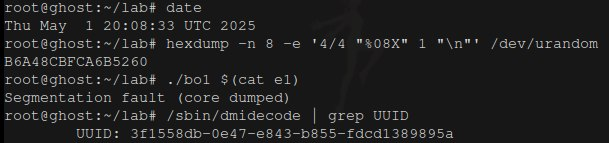
\includegraphics[scale=1]{./images/4.jpg}
\end{center}

\begin{enumerate}[resume]
	\item Процесс отладки уязвимой программы в gdb. По скриншоту можно увидеть, что адрес возврата \texttt{0x0804919f}.
\end{enumerate}

\begin{center}
	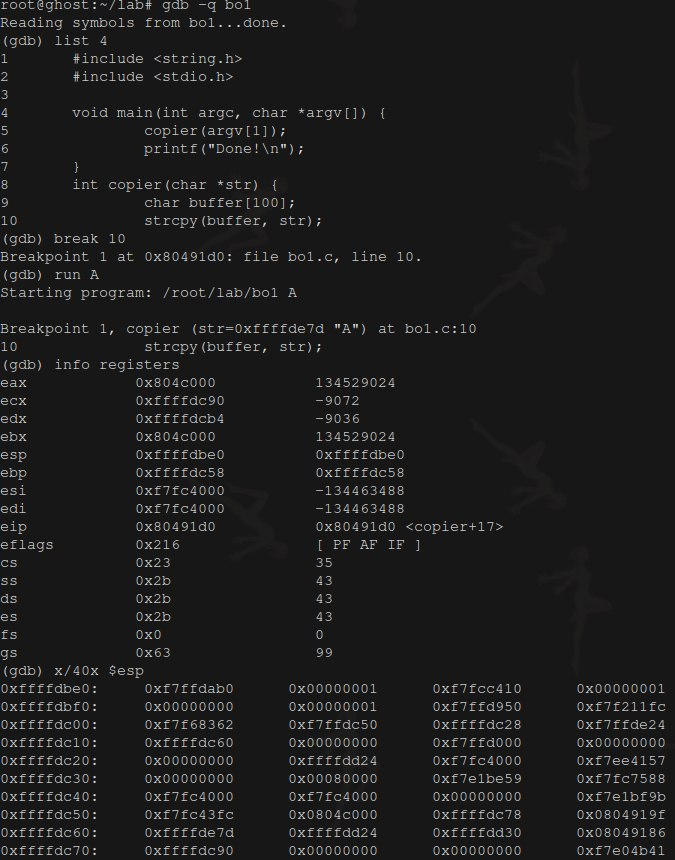
\includegraphics[scale=1]{./images/5.jpg}
\end{center}

\begin{enumerate}[resume]
	\item Прикладываю распечатку своего стека при вводе 116 букв A. По возникновению ошибки \texttt{Segmentaion Fault} при измененной длине входящего сообщения можно предположить изменение адреса возврата. Адрес возврата можно увидеть в GDB при запуске (в нашем случае он стал равен \texttt{0x41414141}).
\end{enumerate}

\begin{center}
	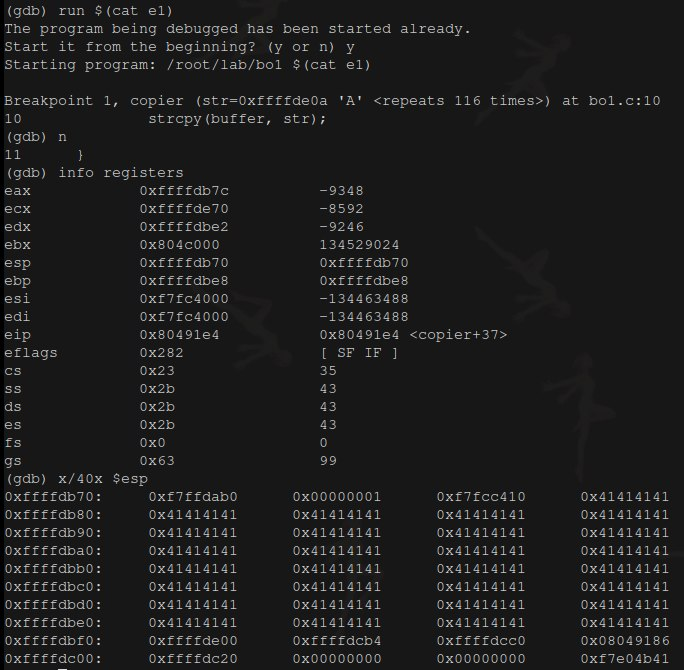
\includegraphics[scale=1]{./images/6.jpg}
\end{center}

\begin{enumerate}[resume]
	\item Запуск с подменным адресом возврата на \texttt{0x31323334}.
\end{enumerate}

\begin{center}
	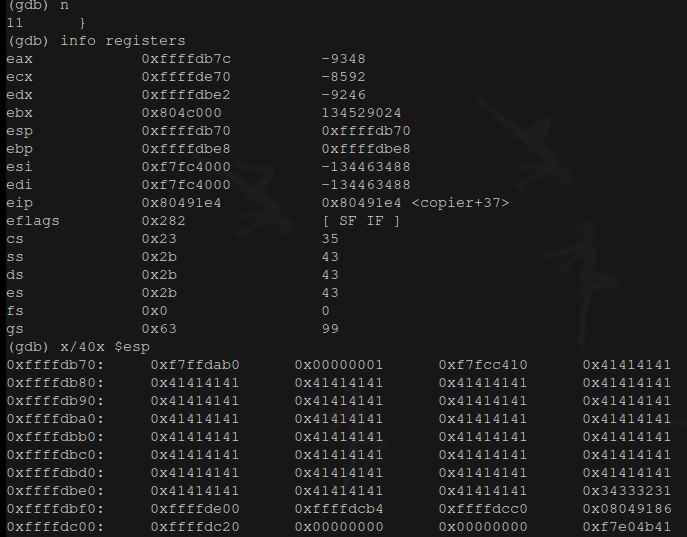
\includegraphics[scale=1]{./images/7.jpg}
\end{center}

\begin{enumerate}[resume]
	\item Прикладываю скриншот с распечаткой стека моей машины(произошел непланированный перезапуск виртуальной мащины, поэтому в gdb некоторые адреса поменялись). Мой полученный адрес возврата \texttt{0xbffffc1c}.
\end{enumerate}

\begin{center}
	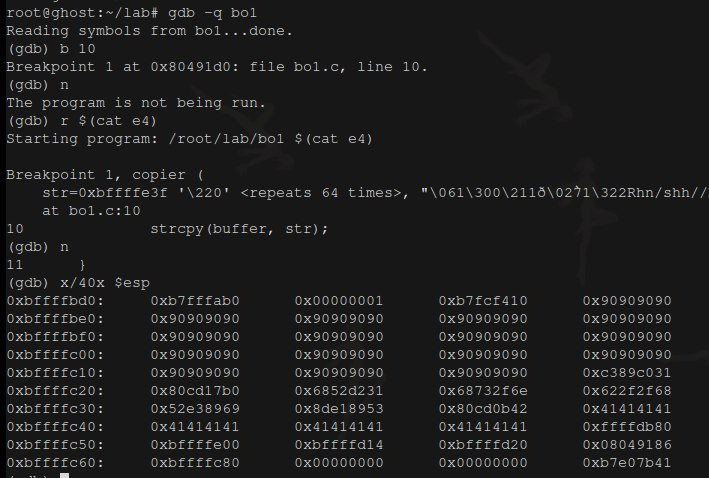
\includegraphics[scale=1]{./images/8.jpg}
\end{center}

\begin{enumerate}[resume]
	\item Ура, мы получили терминал и выполнили команду date.
\end{enumerate}

\begin{center}
	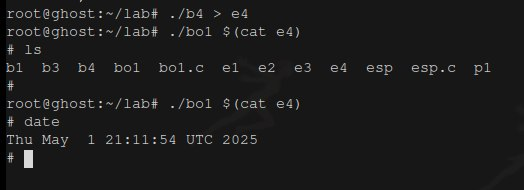
\includegraphics[scale=1]{./images/9.jpg}
\end{center}

\begin{enumerate}[resume]
	\item Чтобы правильно подобрать размер инжектированного кода самый надеждный способ гененрировать уникальные куски входных данных(например, последовательность де Брёйна) по размеру указателя, а затем указать строку подлиньше. Так же можно сделать это статически без запуска программы: достаточно знать структуру стека.
\end{enumerate}

\begin{enumerate}[resume]
	\item При попытке воспроизвести (после включения обратно ASLR) уязвимости получаем ожидаемый \texttt{Segmentation fault}.
\end{enumerate}

\begin{center}
	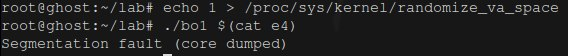
\includegraphics[scale=1]{./images/10.jpg}
\end{center}

\begin{enumerate}[resume]
	\item На этапе компиляции можно было установить канарейку поверх стека. На моменте написания кода можно было использовать strncpy с количественным указанием размера считываемого буфера. На этапе проектирования можно было выбрать другой язык программирования для этой программы. Если сделали без митигаций и обработки ошибок на Си, то на этапе перед релизом можно было отправить на тестирование или подвергнуть фаззинг-тестированию.
\end{enumerate}

\end{document}
